% ------------------------------------------------------------------------
% ------------------------------------------------------------------------
% abnTeX2: Modelo de Trabalho Academico (tese de doutorado, dissertacao de
% mestrado e trabalhos monograficos em geral) em conformidade com 
% ABNT NBR 14724:2011: Informacao e documentacao - Trabalhos academicos -
% Apresentacao
% ------------------------------------------------------------------------
% ------------------------------------------------------------------------

\documentclass[
	% -- opções da classe memoir --
	10pt,				% tamanho da fonte
%	openright,			% capítulos começam em pág ímpar (insere página vazia caso preciso)
%	twoside,			% para impressão em verso e anverso. Oposto a oneside
	oneside,
	a4paper,			% tamanho do papel. 
	% -- opções da classe abntex2 --
	%chapter=TITLE,		% títulos de capítulos convertidos em letras maiúsculas
	%section=TITLE,		% títulos de seções convertidos em letras maiúsculas
	%subsection=TITLE,	% títulos de subseções convertidos em letras maiúsculas
	%subsubsection=TITLE,% títulos de subsubseções convertidos em letras maiúsculas
	% -- opções do pacote babel --
  % adicionar idiomas para hifenização.
  % the last is the main language of the document
%	french,				% idioma adicional para hifenização
%	spanish,			% idioma adicional para hifenização
	brazil,
	english
	]{abntex2}

% ---
% PACOTES
% ---

% ---
% Pacotes fundamentais 
% ---
\usepackage{lmodern}			% Usa a fonte Latin Modern			
\usepackage[T1]{fontenc}		% Selecao de codigos de fonte.
\usepackage[utf8]{inputenc}		% Codificacao do documento (conversão automática dos acentos)
\usepackage{lastpage}			% Usado pela Ficha catalográfica
\usepackage{indentfirst}		% Indenta o primeiro parágrafo de cada seção.
\usepackage{color}				% Controle das cores
\usepackage{graphicx}			% Inclusão de gráficos
\usepackage{microtype} 			% para melhorias de justificação

\setfloatadjustment{figure}{\centering} % auto centers images (comes from memoir, abntex is based on it)
\DeclareGraphicsExtensions{.pdf,.png,.jpg}

% ---
		
% ---
% Pacotes adicionais, usados apenas no âmbito do Modelo Canônico do abnteX2
% ---
\usepackage{lipsum}				% para geração de dummy text
% ---

% ---
% Pacotes de citações
% ---
%\usepackage[brazilian,hyperpageref]{backref}	 % Paginas com as citações na bibl
\usepackage[alf]{abntex2cite}	% Citações padrão ABNT

% --- 
% CONFIGURAÇÕES DE PACOTES
% --- 

%% ---
%% Configurações do pacote backref
%% Usado sem a opção hyperpageref de backref
%\renewcommand{\backrefpagesname}{Citado na(s) página(s):~}
%% Texto padrão antes do número das páginas
%\renewcommand{\backref}{}
%% Define os textos da citação
%\renewcommand*{\backrefalt}[4]{
%	\ifcase #1 %
%		Nenhuma citação no texto.%
%	\or
%		Citado na página #2.%
%	\else
%		Citado #1 vezes nas páginas #2.%
%	\fi}%
%% ---

% ---
% Informações de dados para CAPA e FOLHA DE ROSTO
% ---
\titulo{A Domain Specific Language for OntoUML}
\autor{Reinaldo de Souza Junior}
\local{Vitória - ES, Brasil}
\data{2013}
\orientador{Prof. Dr. João Paulo Andrade Almeida}
%\coorientador{Equipe \abnTeX}
\instituicao{%
  Universidade Federal do Espírito Santo -- UFES
  \par
  Centro Tecnológico
  \par
  Departamento de Ciência da Computação
}
\tipotrabalho{Monografia}
% O preambulo deve conter o tipo do trabalho, o objetivo, 
% o nome da instituição e a área de concentração 
\preambulo{
  Monografia apresentada ao curso de Ciência da Computação
  do Centro Tecnológico da Universidade Federal do Espírito Santo,
  como requisito parcial para obtenção do título de Bacharel em Ciência da Computação.
%  Orientador: \imprimirorientador
}
% ---


% ---
% Configurações de aparência do PDF final

% alterando o aspecto da cor azul
\definecolor{blue}{RGB}{41,5,195}

% informações do PDF
\makeatletter
\hypersetup{
     	%pagebackref=true,
		pdftitle={\@title}, 
		pdfauthor={\@author},
    	pdfsubject={\imprimirpreambulo},
	    pdfcreator={LaTeX with abnTeX2},
		pdfkeywords={abnt}{latex}{abntex}{abntex2}{trabalho acadêmico}, 
		colorlinks=true,       		% false: boxed links; true: colored links
    	linkcolor=blue,          	% color of internal links
    	citecolor=blue,        		% color of links to bibliography
    	filecolor=magenta,      		% color of file links
		urlcolor=blue,
		bookmarksdepth=4
}
\makeatother
% --- 

% --- 
% Espaçamentos entre linhas e parágrafos 
% --- 

% O tamanho do parágrafo é dado por:
\setlength{\parindent}{1.3cm}

% Controle do espaçamento entre um parágrafo e outro:
\setlength{\parskip}{0.2cm}  % tente também \onelineskip

% ---
% compila o indice
% ---
\makeindex
% ---

% ----
% Início do documento
% ----
\begin{document}

% Retira espaço extra obsoleto entre as frases.
\frenchspacing

% ----------------------------------------------------------
% ELEMENTOS PRÉ-TEXTUAIS
% ----------------------------------------------------------
% \pretextual

% ---
% Capa
% ---
\imprimircapa
% ---

% ---
% Folha de rosto
% (o * indica que haverá a ficha bibliográfica)
% ---
\imprimirfolhaderosto*
% ---

% ---
% Inserir a ficha bibliografica
% ---

% Isto é um exemplo de Ficha Catalográfica, ou ``Dados internacionais de
% catalogação-na-publicação''. Você pode utilizar este modelo como referência. 
% Porém, provavelmente a biblioteca da sua universidade lhe fornecerá um PDF
% com a ficha catalográfica definitiva após a defesa do trabalho. Quando estiver
% com o documento, salve-o como PDF no diretório do seu projeto e substitua todo
% o conteúdo de implementação deste arquivo pelo comando abaixo:
%
% \begin{fichacatalografica}
%     \includepdf{fig_ficha_catalografica.pdf}
% \end{fichacatalografica}
%\begin{fichacatalografica}
%	\vspace*{\fill}					% Posição vertical
%	\hrule							% Linha horizontal
%	\begin{center}					% Minipage Centralizado
%	\begin{minipage}[c]{12.5cm}		% Largura
%	
%	\imprimirautor
%	
%	\hspace{0.5cm} \imprimirtitulo  / \imprimirautor. --
%	\imprimirlocal, \imprimirdata-
%	
%	\hspace{0.5cm} \pageref{LastPage} p. : il. (algumas color.) ; 30 cm.\\
%	
%	\hspace{0.5cm} \imprimirorientadorRotulo~\imprimirorientador\\
%	
%	\hspace{0.5cm}
%	\parbox[t]{\textwidth}{\imprimirtipotrabalho~--~\imprimirinstituicao,
%	\imprimirdata.}\\
%	
%	\hspace{0.5cm}
%		1. Conceptual Modeling
%		2. OntoUML
%		I. Prof. Dr. João Paulo Andrade Almeida
%		II. Universidade Federal do Espírito Santo
%    III. TITULO\\
%	
%	\hspace{8.75cm} CDU 02:141:005.7\\
%	
%	\end{minipage}
%	\end{center}
%	\hrule
%\end{fichacatalografica}
% ---

% ---
% Inserir errata
% ---
%\begin{errata}
%Elemento opcional da \citeonline[4.2.1.2]{NBR14724:2011}. Exemplo:
%
%\vspace{\onelineskip}
%
%FERRIGNO, C. R. A. \textbf{Tratamento de neoplasias ósseas apendiculares com
%reimplantação de enxerto ósseo autólogo autoclavado associado ao plasma
%rico em plaquetas}: estudo crítico na cirurgia de preservação de membro em
%cães. 2011. 128 f. Tese (Livre-Docência) - Faculdade de Medicina Veterinária e
%Zootecnia, Universidade de São Paulo, São Paulo, 2011.
%
%\begin{table}[htb]
%\center
%\footnotesize
%\begin{tabular}{|p{1.4cm}|p{1cm}|p{3cm}|p{3cm}|}
%  \hline
%   \textbf{Folha} & \textbf{Linha}  & \textbf{Onde se lê}  & \textbf{Leia-se}  \\
%    \hline
%    1 & 10 & auto-conclavo & autoconclavo\\
%   \hline
%\end{tabular}
%\end{table}
%
%\end{errata}
% ---

% ---
% Inserir folha de aprovação
% ---

% Isto é um exemplo de Folha de aprovação, elemento obrigatório da NBR
% 14724/2011 (seção 4.2.1.3). Você pode utilizar este modelo até a aprovação
% do trabalho. Após isso, substitua todo o conteúdo deste arquivo por uma
% imagem da página assinada pela banca com o comando abaixo:
%
% \includepdf{folhadeaprovacao_final.pdf}
%
\begin{folhadeaprovacao}

  \begin{center}
    {\ABNTEXchapterfont\large\imprimirautor}

    \vspace*{\fill}\vspace*{\fill}
    \begin{center}
      \ABNTEXchapterfont\bfseries\Large\imprimirtitulo
    \end{center}
    \vspace*{\fill}
    
    \hspace{.45\textwidth}
    \begin{minipage}{.5\textwidth}
        \imprimirpreambulo
    \end{minipage}%
    \vspace*{\fill}
   \end{center}
        
   Trabalho aprovado. \imprimirlocal, ?? de dezembro de 2013:

   \assinatura{\textbf{\imprimirorientador} \\ Orientador} 
   \assinatura{\textbf{Professor} \\ Convidado 1}
   \assinatura{\textbf{Professor} \\ Convidado 2}
   %\assinatura{\textbf{Professor} \\ Convidado 3}
   %\assinatura{\textbf{Professor} \\ Convidado 4}
      
   \begin{center}
    \vspace*{0.5cm}
    {\large\imprimirlocal}
    \par
    {\large\imprimirdata}
    \vspace*{1cm}
  \end{center}
  
\end{folhadeaprovacao}
% ---

% ---
% Dedicatória
% ---
%\begin{dedicatoria}
%   \vspace*{\fill}
%   \centering
%   \noindent
%   \textit{Foo} \vspace*{\fill}
%\end{dedicatoria}
% ---

% ---
% Agradecimentos
% ---
\begin{agradecimentos}
%
\end{agradecimentos}
% ---

% ---
% Epígrafe
% ---
%\begin{epigrafe}
%    \vspace*{\fill}
%	\begin{flushright}
%		\textit{``Não vos amoldeis às estruturas deste mundo, \\
%		mas transformai-vos pela renovação da mente, \\
%		a fim de distinguir qual é a vontade de Deus: \\
%		o que é bom, o que Lhe é agradável, o que é perfeito.\\
%		(Bíblia Sagrada, Romanos 12, 2)}
%	\end{flushright}
%\end{epigrafe}
% ---

% ---
% RESUMOS
% ---

% resumo em português
\setlength{\absparsep}{18pt} % ajusta o espaçamento dos parágrafos do resumo
\begin{resumo}
 Essa monografia provê uma sintaxe textual para a criação de modelos conceituais
 baseados numa linguagem de modelagem filosoficamente e cognitivamente bem-fundada,
 chamada OntoUML, bem como um editor para o uso desta linguagem.
%
 Primeiramente, revisamos as restrições de integridade contidas no metamodelo
 da linguagem OntoUML e as adequamos de modo a ser compatível com o ferramental atual.
%
 Em seguida, propomos uma sintaxe concreta textual (uma linguagem específica de domínio, DSL)
 para representar os conceitos existentes no metamodelo.
%
 Na sequência, desenvolvemos um editor textual para que usuários possam criar e
 manipular modelos OntoUML por meio da DSL proposta.
%
 Objetivo é criar uma linguagem textual que represente os conceitos da linguagem
 OntoUML e fornecer a ferramenta necessária para seu uso.
%
 Portanto, nesse trabalho propomos uma sintaxe concreta para a linguagem OntoUML
 e provemos uma ferramenta que possibilita a edição, validação sintática e
 transformação de modelos.
%
% Segundo a \citeonline[3.1-3.2]{NBR6028:2003}, o resumo deve ressaltar o
% objetivo, o método, os resultados e as conclusões do documento. A ordem e a extensão
% destes itens dependem do tipo de resumo (informativo ou indicativo) e do
% tratamento que cada item recebe no documento original. O resumo deve ser
% precedido da referência do documento, com exceção do resumo inserido no
% próprio documento. (\ldots) As palavras-chave devem figurar logo abaixo do
% resumo, antecedidas da expressão Palavras-chave:, separadas entre si por
% ponto e finalizadas também por ponto.

 \textbf{Palavras-chaves}: OntoUML. linguagem específica de domínio. Eclipse. Xtext.
\end{resumo}

% resumo em inglês
\begin{resumo}[Abstract]
 \begin{otherlanguage*}{english}
   This work provides both a textual sintax to creating conceptual models 
   based on a philosophically and cognitively well-founded modeling language,
   named OntoUML, and an editor to the language itself.
%
   First, we review the integrity constraints contained in the language's metamodel
   and we suit them to be compatible with the current tooling.
%
   Then, we propose a textual concrete syntax (a domain specific language, DSL)
   to represent the concepts existing in the metamodel.
%
   In the sequel, we design a textual editor based on the Eclipse platform
   to allow users to create and manipulate OntoUML models using the proposed DSL.
%
   The goal is to create a textual language that represents the concepts of
   the OntoUML language and provide a tool needed for its use.
%
   Therefore, in this work we propose a concrete sintax to the OntoUML language
   and provide a tool which support the editing, syntax validation and
   transformation of models.

   \textbf{keywords}: OntoUML. domain specific language. Eclipse. Xtext.
 \end{otherlanguage*}
\end{resumo}
% ---

% ---
% inserir lista de ilustrações
% ---
%\pdfbookmark[0]{\listfigurename}{lof}
%\listoffigures*
%\cleardoublepage
% ---

% ---
% inserir lista de tabelas
% ---
%\pdfbookmark[0]{\listtablename}{lot}
%\listoftables*
%\cleardoublepage
% ---

% ---
% inserir lista de abreviaturas e siglas
% ---
%\begin{siglas}
%  \item[Fig.] Area of the $i^{th}$ component
%  \item[456] Isto é um número
%  \item[123] Isto é outro número
%  \item[lauro cesar] este é o meu nome
%\end{siglas}
% ---

% ---
% inserir lista de símbolos
% ---
%\begin{simbolos}
%  \item[$ \Gamma $] Letra grega Gama
%  \item[$ \Lambda $] Lambda
%  \item[$ \zeta $] Letra grega minúscula zeta
%  \item[$ \in $] Pertence
%\end{simbolos}
% ---

% ---
% inserir o sumario
% ---
\pdfbookmark[0]{\contentsname}{toc}
\tableofcontents*
\cleardoublepage
% ---

% ----------------------------------------------------------
% ELEMENTOS TEXTUAIS
% ----------------------------------------------------------
\textual

%  ---------------------------------------------------------
%  Proposed structure
%  ---------------------------------------------------------
%  
%  1 – Introdução
%    Motivação de modelagem conceitual, OntoUML
%    Motivação de emprego de uma notação textual (conveniente para experts)
%    Objetivo: definição de uma notação textual com suporte ferramental
%    Abordagem: desenvolvimento orientado a modelos com ferramental Eclipse
%  2 – Tecnologias Empregadas
%    OntoUML
%    Eclipse
%    ECORE/EMF
%    OCL
%    Xtext
%  4 – Sintaxe concreta
%    Requisitos
%    Apresentação da gramática com exemplos
%    Port de restrições OCL de refontouml para OntoUMLprime 
%  5 – Desenvolvimento do Editor
%    Justificar e documentar escolhas de implementação	
%    Transformação para RefOntoUML
%  6 – Conclusões


% ----------------------------------------------------------
% Introdução
% ----------------------------------------------------------
% \chapter*[Introduction]{Introduction}
% \addcontentsline{toc}{chapter}{Introduction}

% Can't see how the introduction should be different from CARRARETTO R., 2010
\chapter[Introduction]{Introduction}

Information is an abundant, ubiquitous and precious resource. Most of the information available to us is in computer-based forms, such as files and databases. Thus, the task of computer scientists is to develop theories, tools and techniques for managing this information and making it useful. To use information, one needs to represent it, capturing its meaning and inherent structure. Such representations are important for communicating information between people, but also for building information systems that manage and exploit this information in the performance of useful tasks \cite{mylopoulos98}.
%
A particular important activity to arrive at such representations is conceptual modeling, which is defined as “the activity of formally describing some aspects of the physical and social world around us for purposes of understanding and communication. Moreover, it supports structuring and inferential facilities that are psychologically grounded. After all, the descriptions that arise from conceptual modeling activities are intended to be used by humans, not machines” \cite{mylopoulos92}.

As clearly stated by \citeauthor{carraretto10}:
(Is it bad to quote someone else's introduction on what should be my own introduction?)
%
\begin{quotation}
As any pragmatic subject, conceptual modeling can profit from tool support to complete its purpose. Since conceptual models are concrete artifacts, they must exist in the physical world. Therefore, in order to obtain such artifacts, users primarily need a tool for creating and editing the constructs of a modeling language. Besides editing, there is a variety of manipulations that can be done with a model (henceforth, model manipulation) such as analysis of its content, syntactic and semantic validation, interchange between conceptual modeling tools, persistence in different formats, generation of textual documentation, transformations to different modeling languages, etc.

Although it is possible to create conceptual models using a pen and a piece of paper (or, perhaps, cave walls and red ochre), users desire the usability and flexibility provided by computer-based tools. However, even those types of tools can be built in an ad hoc manner. For instance, many of the model manipulation activities can be done in different tools that do not share any implementation aspect and, as a consequence, lack integration and reusability. Such situation impacts both users and developers. On one hand, users cannot perform their modeling activities easily, since there is no integration between tools. On the other hand, developers perform extra tasks every time a new tool to support some modeling activity has to be developed, because there is no reusability.
\end{quotation}

We address these issues in this work by providing an organized infrastructure for conceptual modeling that integrates many modeling activities, such as model editing and manipulation, and promotes reusability of modeling components.
%
More specifically, we
build on top of Carraretto's work \cite{carraretto10} to
give tool support for a well-founded conceptual modeling language, namely OntoUML \cite{guizzardi05}, providing:
% \begin{itemize}[nolistsep] \firmlists* \tightlist
\begin{itemize}[nolistsep]{\topsep=0em\partopsep=0em} \tightlist
  \item a reference metamodel to be the core of model manipulation;
  \item a textual language to describe OntoUML models;
  \item a textual editor for constructing models, and also
  \item syntax validation by means of OCL syntactical constraints.
\end{itemize}
%
Thus, we provide a modeling infrastructure for OntoUML.

%Both reference metamodel and syntactical constraints are derived from Carraretto's work \cite{carraretto10}.
%

% \setcounter{chapter}{1}
\section{Background}

% Abstract
% My work is a textual concrete syntax for a shared abstract syntax.
% The OntoUML language has a few different metamodels:
% Benevides' metamodel is polluted by GMF concepts and Carraretto's metamodel is
% polluted by UML2 concepts. They both are not good fits for a foundational
% metamodel.
% My work provides a foundational metamodel that acts as abstract syntax for a
% conceptualization of a foundational ontology (UFO). And also provides a textual
% concrete syntax for this foundational metamodel. And, finally, transformations
% from this metamodel to the other metamodels.

% 1. What is a metamodel and why it is needed.

% Conceptualization -> Unified Foundational Ontlogy
% Modeling Language -> OntoUML (in one of its abstract syntaxes)
%                   -> it is "used to compose" a model by means of a corresponding
%                      concrete syntax

Abstractions of a given portion of reality are constructed in terms of
concepts, i.e., abstract representations of certain aspects of entities that
exist in that domain.
%
\emph{Conceptualization} is the set of concepts used to articulate abstractions
of state of affairs in a given domain. The abstraction of a given portion of
reality articulated according to a domain conceptualization is termed here a
\emph{domain abstraction}.
%
Conceptualizations and domain abstractions are abstract entities that only exist
in the mind of the user or a community of users of a language. In order to be
documented, communicated and analyzed, these entities must be captured
in terms of some concrete artifact.
%
The representation of a conceptual model is named here a \emph{model}.
Moreover, in order to represent a model, a \emph{modeling language} is necessary.
%
The relation between conceptualization, domain abstraction, modeling language and
models is depicted in figure~\ref{fig:materializing_concepts} below.
\cite{carraretto10} and \cite{guizzardi05}.

\begin{figure}[here]
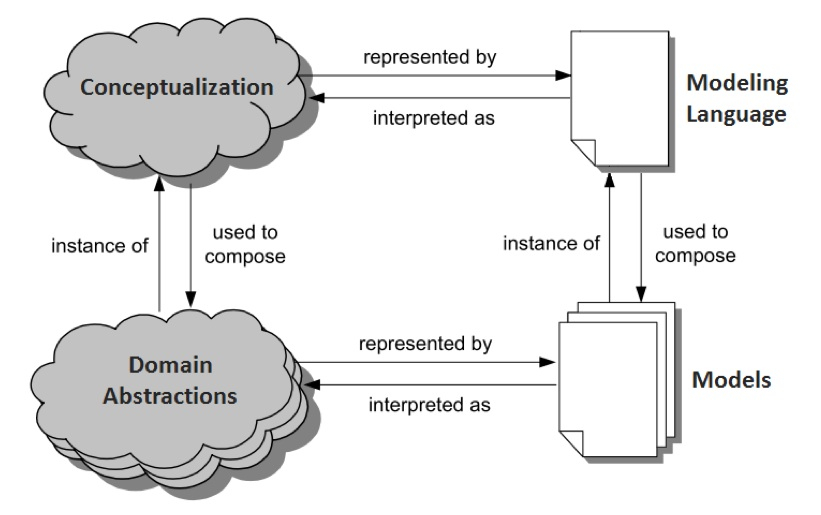
\includegraphics[width=0.8\textwidth]{images/materializing_concepts}
\caption{Relation between conceptualization, domain abstraction, modeling language and
models}
\label{fig:materializing_concepts}
\end{figure}

According to \citeonline[p. 3]{harel_rumpe00},
"A \emph{language} consists of a syntactic notation (syntax) which is a possibly
infinite set of elements that can be used in the communication, together with
their meaning (semantics)."

The syntactic notation can be divided in two parts: the \emph{abstract syntax}
and the \emph{concrete syntax}.
%
The abstract syntax is responsible for defining the elements of the language and
the rules for relating them in valid expressions.
%
The concrete syntax is responsible for defining a concrete representation of each
element and relation previously defined so they can be manipulated to create valid
expressions. \cite{harel_rumpe00}

A semantic definition for a language, or simply a \emph{semantics}, consists of
two parts: a \emph{semantic domain}, and a \emph{semantic mapping} from the syntax
to the semantic domain.

Similarly to Guizzardi's definition of \emph{conceptualization}, Harel and Rumpe
define the \emph{semantic domain} as the specification of "\ldots the very concepts
that exist in the universe of discourse. It is an abstraction of reality, describing
the important aspects of the systems that we are interested in developing. It is
also a prerequisite for comparing different semantic defitions."

Although, the semantic domain is defined for describing the meaning of a notation,
the definition of the semantic domain is normally independent of the notation.
This allows to "reuse" the semantic domain for other notations. \cite{harel_rumpe00}

% TODO: I could not find a sumrized version of this definition on the original
% source, so I'm citing Carraretto's summary
A \emph{foundational ontology} is a representation of theories that describe
knowledge about reality in a way, which is independent of language, of particular
states of affairs (states of the world), and epistemic states of knowledgeable agents.
In other words, a foundational ontology is a domain-independent philosophically
and cognitively well-founded system of real-world categories. It deals with formal
aspects of objects irrespective of their particular nature, including concepts
from theory of parts, theory of wholes, types and instantiation, identity,
dependence, unity. Furthermore, a foundational ontology can be used to provide
real-world semantics for general conceptual modeling languages, and to constrain
the possible interpretations of their modeling primitives. \cite{carraretto10}

% -----------------------------------------------------------------------------
Now, we are able to contextualize this work in terms of the concepts previously
presented.
%
% ------------------------------------------------------------------------------
% ALternative contextualization
% ------------------------------------------------------------------------------
%First, our \emph{conceptualization} encompasses the concepts of a unified foundational
%ontology (UFO) defined in \cite{guizzardi05}.
%Furthermore, we represent the concepts of the UFO in a textual modeling language
%containing both abstract syntax (metamodel) and concrete syntax (textual DSL).
%
In this work, we provide a full implementation of a modeling language, containing
both its abstract syntax (metamodel) and concrete syntax (textual DSL).
Despite having different abstract and concrete syntaxes, the proposed language is
compatible with the OntoUML language because they share the same semantic domain
(conceptualization): a unified foundational ontology (UFO) defined in \cite{guizzardi05}.
% -----------------------------------------------------------------------------

\section{Motivation and Goals}

Although tool support for OntoUML conceptual models has already been developed
in \cite{carraretto10}, where a tool for building and validating the syntax
of OntoUML conceptual models were provided - as well as a \emph{reference metamodel}
for OntoUML, in our work we address some problems related to the author’s approach.
%
Basically, those problems are related to his metamodel implementation.

First, it uses a fully-compliant UML 2.0 metamodel implementation as a foundation.
Because of this, the metamodel is too polluted with UML constraints which are not
strictly necessary to create well-founded conceptual models.
%
Second, its generated plugins have dependencies which were deprecated on recent
versions of Eclipse, which constrains the adoption of the tool as well as its
integration with more recent tools based on Eclipse (Xtext in our case).
%
% TODO: Find an official statement about the deprecation of this article
% http://www.eclipse.org/articles/article.php?file=Article-EMF-Codegen-with-OCL/index.html
%
And third, the OCL syntactical constraints are defined in terms of annotations in
the same metamodel. It makes hard to visualize, manipulate and reuse the constraints.

Consequently, one goal is to develop a metamodel that: is independent of UML 2.0;
is compatible with the latest versions of the Eclipse Modeling package;
and has the metamodel specification and syntactical constraints separated but
still integrated.

Another goal is to propose a textual concrete syntax for the OntoUML language and
provide tooling to manipulate models specified in this language.
%
% TODO: Maybe add transformations as goals, and then make the transformations
% Alternatively, we also provide a transformation from the reference metamodel developed in (Carraretto, 2010) to our metamodel. This way, users can choose any of the two editors and still enjoy the advantages of our metamodel.

\section{Approach and Structure}

In order to achieve our goals, we use the tools encompassed in the Eclipse Modeling
Project. The Eclipse Modeling Project focuses on the evolution and promotion of
model-based development technologies
within the Eclipse community by providing a unified set of modeling frameworks,
tooling, and standards implementations [built on top of the Eclipse software
development environment]\footnote{http://www.eclipse.org/modeling/}.

Another important aspect is that Eclipse has an extensible plug-in system that
allows us to provide new functionalities on top of the runtime system.
Moreover, Eclipse is free and open source software.

%TODO
TODO: Talk about the structure, describing what each chapter contains.

\chapter{Modeling Infrastructure}

%\chapter{A concrete syntax for the reference metamodel}

In this chapter, we present the general aspects of our modeling infrastructure by
describing its elements, the technologies in use and their relations.

First, we assess the alleged suitability to reuse of the reference metamodel
proposed by \cite{carraretto10}.
%
%First, we use the current tooling provided by the Eclipse Modeling Project to
%build a textual concrete syntax for the abstract syntax defined by the reference
%metamodel.
%
Then we document the problems faced during this assessment and identify some
properties that are desirable to a metamodel indended for this level of reuse.
Finally, we propose our new infrastructure.

In addition, we provide general details about the tools used to implement the infrastructure.

\section{Previous infrastructure}

%TODO
** make my point and include excerpts from my first frustration\footnote{https://github.com/juniorz/ontouml\_editor/}

** stress the properties in primeontouml that made it easy and suitable for reuse.

Before our work, tool support for OntoUML was already provided in both
\cite{benevides10} and \cite{carraretto10}. Each work provide an editor for
OntoUML, built on top of Eclipse software development environment.

In this context, an editor is a software that allows the user to manipulate the
concrete syntax of the language by relating the elements that compose it
according to the abstract syntax specification,
also called the metamodel of the language.

That said, an editor is responsible for providing to the user an interface to
manipulate instances of the metamodel (also called, models) by means of a
concrete syntax.

In \cite{carraretto10}, a fully-compliant UML 2.0 metamodel is proposed to
address the problems existing in \cite{benevides10} and also
"\ldots be used as a reference metamodel for any model manipulation purposes
(including abstract syntax validation).".
However, Carrareto's work also carries its own issues with respect to reuse.

%TODO: describe what we did
** Should we mention that we tried to create a concrete syntax for this reference
metamodel and describe how we did it, and THEN talk about the problems we found?

First, the reference metamodel is based on the Eclipse implementation of the UML
Superstructure (included in EMF 2.5) metamodel. That is, the metamodel was built
in terms of concepts from the metamodel of UML.

For example, every association in UML has properties such navigability and ownership
which are defined by a combination of three meta-properties (ownedEnd, memberEnd
and navigableOwnedEnd).
%
"A navigable end of an association means that it is intended to be traversed at
runtime from objects participating in links at the other end(s) of the association
to objects participating in links at the navigable end.
This is independent of ownership of the end." \cite{UML20}
%
Such concepts are closely related to implementation details and have no relevance
in the field of strictly conceptual models.
%
This fact also imposes some restrictions to the concrete syntax due to the way
the Xtext grammar definition relates to the language metamodel, as can be seen in
the following example:

\begin{verbatim}
role Parent : Person { }
role Offspring : Person { }
relator Registration { }

mediation M1 {
  property m11 (Registration);  //memberEnd
  property m12 (Offspring);     //memberEnd
  memberEnd m11, m12;
}

mediation M2 {
  property m21 (Registration);  //memberEnd
  property m22[1,2] (Parent);   //memberEnd
  memberEnd m21, m22;
}
\end{verbatim}

Both mediations (\emph{M1} and \emph{M2}) are simply associations between the roles
and their relator but, due the presence of the extra ownedEnd and memberEnd meta
atributes (inherited from the UML metamodel) and the fact that the syntactical
constraints were written in terms of these same attributes, forced the mediation
syntax to hold a notation excessively verbose.
%
%

By specifying the concepts of the unified foundational ontology without referring
to UML concepts, we were able to represent the same concept more clearly:

\begin{verbatim}
RelatorUniversal Registration {
  mediates Offspring[1..1];
  mediates Parent[1..2];
}
\end{verbatim}

% TODO: ask the forum for a "official name" for this approach.
% I don't think it is called OCLInEcore
% http://web.archiveorange.com/archive/v/p3ScLAH4y6yBY6KhWy3W
Second, it uses a technology to support the usage of OCL constraints which requires
the constraints to be embedded into the metamodel by the means of EAnnotations.
Then, these EAnnotations are used by EMF to enhance the model validator.

Once again, due the way the Xtext editor delegates validation to the EMF model and
the lack of features in the OCLInEcore implementation, the generated error messages
were not as clean and useful as desired, to the extent of misleading the user
regarding the cause of the error.

** Include a screenshot

%TODO: confirm this, by installing Eclipse Helios, Indigo, Juno, Kepler
In addition to that, the OCL plugin in use is deprecated in Eclipse versions Helios
and later and the provided workaround\footnote{http://wiki.eclipse.org/MDT/OCL/FAQ\#How\_do\_I\_workaround\_org.eclipse.emf.ocl\_deprecation\_in\_Helios\_and\_later.3F} compromises the installation, making impossible the integration
of the tool with other components from the Eclipse Modeling Project.

% http://help.eclipse.org/juno/topic/org.eclipse.ocl.doc/help/Integration.html?cp=49_1_7_1#Integration-Messages
We also wanted to use custom validation messages for OCL and that was not possible
with the Indigo Release (or older).



%Despite claiming to be free from concrete syntax concerns, the reference metamodel
%is not completely free from concrete syntax concerns (at least it is not concerned
%exclusively with 

%It is not a metamodel exclusively crafted to represent a foundational ontology.
%It is not a faithful representation of the foundational ontology.

We conclude that, as a modeling language, the reference metamodel is not a true
representation of the unified foundational ontology (the conceptualization it represents)
because it is also polluted with concepts from the UML 2.0 metamodel used as its foundation.
Such fact compromises its suitability to reuse, as stated by the \cite{carraretto10} in his work.

%Benevides metamodel has is not free from concrete syntax concerns.
%It has in the same
%concepts of a specific graphical
%Carrareto's reference metamodel is free from concepts of 
%
%Despite being free from concepts of a particular concrete syntax 
%concerns (in the sense that Benevides
%metamodel has concepts 

\section{Our infrastructure}

** Outline how our infrastructure is organized and how it relates with previous works.
** Mention briefly what piece of tech is involved in every part of the infrastructure.

Essentialy, draw a diagram with:
1. Abstract syntax (metamodel + OCL constraints)
2. Concrete syntax (Xtext Grammar)
3. Editor (Xtext Editor)
4. Reference OntoUML and transformations

\chapter{The UFO reference metamodel}

In this chapter, we define the abstract syntax of our language by means of a
metamodel. First, we present the technology used in its construction, then we
explain the metamodel itself. Finally, we discuss the differences between our
metamodel and the former metamodel defined in a previous work.

%abstract syntax of our language by constructing
%a metamodel free (exempt, clear) of the UFO reference metamodel

\section{The Eclipse Modeling Framework}

Eclipse is an open source software project, the purpose of which is to provide
a highly integrated tool platform. The work in Eclipse includes a core project,
which includes a generic framework for tool integration, and a Java development
environment built using it. Other projects extend the core framework to support
specific kinds of tools and development environments.

The Eclipse Modeling Project is the focal point for the evolution and promotion
of model-based development technologies at Eclipse. At its core is the Eclipse
Modeling Framework (EMF) \cite{budinsky09} which provides the basic framework for modeling.

The EMF exploits the facilities provided by Eclipse to make it possible to relate
modeling concepts directly to their implementations, thereby bringing to Eclipse
— and Java developers in general — the benefits of modeling with a low cost of entry.
%
EMF is a framework and code generation facility that allows to define a model in
a specific format (i.e., Java interfaces, UML diagram, or XML Schema) and then
generate any of the others and also the corresponding implementation classes in
an automated fashion.

Another key contribution of EMF to the Eclipse's modeling landscape is the Ecore
metamodeling language: the standard language for defining metamodels in
the Eclipse project. A simplified subset of Ecore is shown in figure~\ref{fig:ecore_fragment}.

An \emph{EClass} is used to represent a modeled class: it has a name, zero or more
attributes, and zero or more references.
\emph{EAttribute} is used to represent a modeled attribute. Attributes have a
name and a type.
\emph{EReference} is used to represent one end of an association between classes.
It has a name, a boolean flag to indicate if it represents containment, and a
reference (target) type, which is another class.
And, finally, \emph{EDataType} is used to represent the type of an attribute.
A data type can be a primitive type like \emph{int} or \emph{float} or an object
type like \emph{java.util.Date}.

\begin{figure}
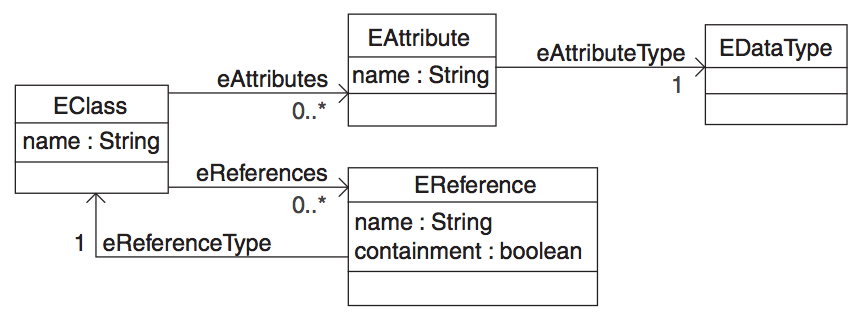
\includegraphics[width=0.8\textwidth]{images/ecore_fragment}
\caption{A simplified subset of the Ecore metamodel \protect\cite{budinsky09}}
\label{fig:ecore_fragment}
\end{figure}

%TODO: Should I add an example? I dont think so.

The most important benefit of EMF, as with modeling in general, is the boost in
productivity that results from automatic code generation. From a single Ecore
model it is possible to generate Java classes and interfaces for every EMF metaclass.

As part of the EMF, the \emph{EMF Validation Framework} provides model validation
capabilities by supporting the evaluation of invariants and constraints via a
validator that is invoked at important moments by an application or at a user's
discretion. \cite{emf_helios_nn}

Prior to EMF version FOO, these invariants and constraints had to be defined
via operations and annotations, respectively. \cite[Chapter~18]{budinsky09}
Then they would be defined as methods during the code generation step and finally
be manually implemented in Java.

%TODO: should I introduce MDT OCL yet?

% This is valid for EMF 2.3 / MDT OCL 1.1
The usage of \emph{Java Emitter Templates} (JET) made possible to integrate the
MDT OCL and the EMF to directly obtain the Java code for validation,
without any post-generation custom code \cite{damus07}.
However, this approach was deprecated with the deprecation of EMF version RAH.

The version BAR of EMF\footnote{part of the Eclipse Helios release} introduced,
the concept of a Validation Delegate, in order to delegate evaluation of invariants and
constraints to an external engine based on a well-defined interface.\cite{emf_helios_nn}
This validation delegate became the standard for extending EMF metamodel validation
capabilities.

%TODO: talk about how we integrated completeOCL constraints in the ecore model.

%TODO: OCL history too?
% http://help.eclipse.org/juno/topic/org.eclipse.ocl.doc/help/Delegates.html?cp=49_5_9
OCLInEcore uses the EMF delegate mechanisms to extend Ecore models with the OCL
engine.

% http://help.eclipse.org/juno/topic/org.eclipse.ocl.doc/help/PivotProgrammersGuide.html#CompleteOCLEObjectValidator
CompleteOCL allows to extend the metamodel with a external OCL document.
We used (If I'm not mistaken) this CompleteOCLEObjectValidator.

% It would be important to talk about all the versions in this paper.
%TODO: Look at Evernote note
In this work, we use the version 4.2 of the Eclipse platform (codename Juno) and
EMF at its version FOO.

\section{Unified Foundational Ontology on Ecore}

%TODO: Talk about how we adapted Carraretto's work to be free of UML concepts
%We already talked about the WHYs.

** aka PrimeontoUML - we need a better name for this, something like Carraretto's reference metamodel.
** What about UFO (reference) metamodel? foundational metamodel, maybe?
** That is because OntoUML is a UML 2.0 Profile that incorporates the foundations captured in the UFO.

We created the UFO reference metamodel in Ecore

\chapter{Textual Concrete Syntax}

\section{Xtext}

\section{Requisites}

\section{Grammar}

\section{Syntactical constraints with CompleteOCL}

The Object Constraint Language (OCL)\cite{OCL20}, is a formal language used to
describe expressions on UML models.

These expressions typically specify invariant conditions that must hold for the
system being modeled or queries over objects described in a model. Note that when
the OCL expressions are evaluated, they do not have side effects (i.e., their
evaluation cannot alter the state of the corresponding executing system).

\chapter{Textual Editor}

\section{Implementation}

\chapter{Transformations}

%-----------------------------------------------------------------
%
%% Approach
%Implementing a language involves several stages:
%1. writing the parser using a compiler generator (like, e.g., Flex \& Bison and ANTLR),
%2. building the abstract syntax tree (AST),
%3. perform all the visits on the AST (e.g., type checking),
%4. and finally generate code into a target language or build the interpreter.
%
%5. Also implement an IDE for the language
% - syntax highlighting
% - code completion, etc.
%
%Eclipse provides a powerful framework for implementing an IDE but it requires lots of programming
%
%Xtext eclipse
%
%1. Write the grammar of the language using an EBNF-like syntax
%2. Xtext generates an ANTLR parser.
%3. During parsing, the AST is generated in the shape of an EMF model

% ----------------------------------------------------------
% PARTE - preparação da pesquisa
% ----------------------------------------------------------
%\part{Preparação da pesquisa}

% ----------------------------------------------------------
% Capitulo com exemplos de comandos inseridos de arquivo externo 
% ----------------------------------------------------------

%\include{abntex2-modelo-include-comandos}

% ----------------------------------------------------------
% Parte de revisão de literatura
% ----------------------------------------------------------
%\part{Referenciais teóricos}

% ---
% Capitulo de revisão de literatura
% ---
%\chapter{Lorem ipsum dolor sit amet}

% ---
%\section{Aliquam vestibulum fringilla lorem}
% ---

%\lipsum[1]

%\lipsum[2-3]

% ----------------------------------------------------------
% Resultados
% ----------------------------------------------------------
%\part{Resultados}

% ---
% primeiro capitulo de Resultados
% ---
%\chapter{Lectus lobortis condimentum}

% ---
%\section{Vestibulum ante ipsum primis in faucibus orci luctus et ultrices
%posuere cubilia Curae}
% ---

%\lipsum[21-22]

% ---
% segundo capitulo de Resultados
% ---
%\chapter{Nam sed tellus sit amet lectus urna ullamcorper tristique interdum
%elementum}
%
%\section{Pellentesque sit amet pede ac sem eleifend consectetuer}
%
%\lipsum[24]

% ---
% Finaliza a parte no bookmark do PDF
% para que se inicie o bookmark na raiz
% e adiciona espaço de parte no Sumário
% ---
%?? \phantompart

% ---
% Conclusão
% ---
\chapter*[Conclusions]{Conclusions}
\addcontentsline{toc}{chapter}{Conclusions}

% ----------------------------------------------------------
% ELEMENTOS PÓS-TEXTUAIS
% ----------------------------------------------------------
\postextual

% ----------------------------------------------------------
% Referências bibliográficas
% ----------------------------------------------------------
%\bibliographystyle{abnt-alf}
\bibliography{paper}

% ----------------------------------------------------------
% Glossário
% ----------------------------------------------------------
%
% Consulte o manual da classe abntex2 para orientações sobre o glossário.
%
%\glossary

% ----------------------------------------------------------
% Apêndices
% ----------------------------------------------------------

% ---
% Inicia os apêndices
% ---
%\begin{apendicesenv}
%
%% Imprime uma página indicando o início dos apêndices
%\partapendices
%
%% ----------------------------------------------------------
%\chapter{Quisque libero justo}
%% ----------------------------------------------------------
%
%\lipsum[50]
%
%% ----------------------------------------------------------
%\chapter{Nullam elementum urna vel imperdiet sodales elit ipsum pharetra ligula
%ac pretium ante justo a nulla curabitur tristique arcu eu metus}
%% ----------------------------------------------------------
%\lipsum[55-57]
%
%\end{apendicesenv}
%% ---


% ----------------------------------------------------------
% Anexos
% ----------------------------------------------------------

%% ---
%% Inicia os anexos
%% ---
%\begin{anexosenv}
%
%% Imprime uma página indicando o início dos anexos
%\partanexos
%
%% ---
%\chapter{Morbi ultrices rutrum lorem.}
%% ---
%\lipsum[30]
%
%% ---
%\chapter{Cras non urna sed feugiat cum sociis natoque penatibus et magnis dis
%parturient montes nascetur ridiculus mus}
%% ---
%
%\lipsum[31]
%
%% ---
%\chapter{Fusce facilisis lacinia dui}
%% ---
%
%\lipsum[32]
%
%\end{anexosenv}

%---------------------------------------------------------------------
% INDICE REMISSIVO
%---------------------------------------------------------------------

%?? \phantompart
\printindex

\end{document}
